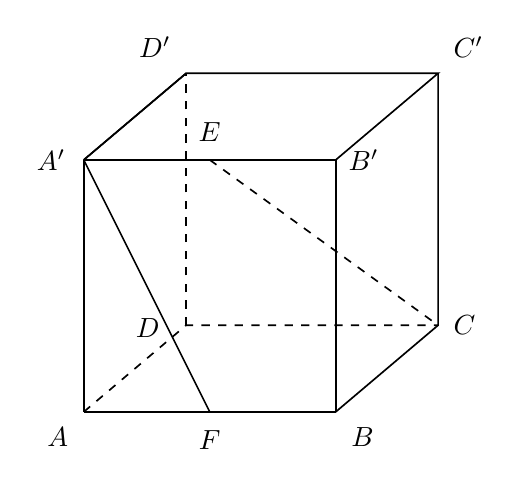
\begin{tikzpicture}[line width=0.6pt, >=stealth]
% cube projection: front A-F-B-B'-A', depth vector d=(1.3,1.1)
\coordinate (A) at (0,0);
\coordinate (F) at (1.6,0);
\coordinate (B) at (3.2,0);
\coordinate (Apr) at (0,3.2);
\coordinate (E) at (1.6,3.2);
\coordinate (Bpr) at (3.2,3.2);
\coordinate (D) at (1.3,1.1);
\coordinate (C) at (4.5,1.1);
\coordinate (Dpr) at (1.3,4.3);
\coordinate (Cpr) at (4.5,4.3);
% solid cube edges
\draw (A) -- (F) -- (B);
\draw (B) -- (Bpr);
\draw (Bpr) -- (E) -- (Apr);
\draw (A) -- (Apr);
\draw (Apr) -- (Dpr) -- (Cpr) -- (Bpr);
\draw (Cpr) -- (C) -- (B);
\draw (Apr) -- (Dpr);
\draw (Apr) -- (F);
% hidden edges (dashed)
\draw[dashed] (A) -- (D) -- (C);
\draw[dashed] (D) -- (Dpr);
\draw[dashed] (E) -- (C);
% labels offset to avoid touching strokes
\node[below left=2pt] at (A) {$A$};
\node[below=3pt] at (F) {$F$};
\node[below right=2pt] at (B) {$B$};
\node[left=3pt] at (Apr) {$A'$};
\node[above=3pt] at (E) {$E$};
\node[right=1pt] at (Bpr) {$B'$};
\node[left=3pt,xshift=-3pt,yshift=-1pt] at (D) {$D$};
\node[right=2pt] at (C) {$C$};
\node[above left=2pt] at (Dpr) {$D'$};
\node[above right=2pt] at (Cpr) {$C'$};
\end{tikzpicture}
